\section{Optimality for constrained problems}

We now investigate how to derive optimality conditions for the problem
\begin{align*}
	(P): ~\mini\braces{f(x) : x \in S}.	
\end{align*}
 
In particular, we are interested in understanding the role that the feasibility set $S$ has on the optimality conditions of constrained optimisation problems in the form of $P$. Let us first define two geometric elements that we will use to derive the optimality conditions for $P$.
%
\begin{definition}[cone of feasible directions]
	Let $S \subseteq \reals^n$ be a nonempty set, and let $\overline{x} \in \clo(S)$. The \emph{cone of feasible directions $D$} at $\overline{x}\in S$ is given by
	$$ 
	D = \braces{d : d \neq 0, \text{ and } \overline{x} + \lambda d \in S \text{ for all } \lambda \in (0,\delta) \text{ for some } \delta > 0}.
	$$
\end{definition}

\begin{definition}[cone of descent directions]
Let $S \subseteq \reals^n$ be a nonempty set, $f: \reals^n \rightarrow \reals$, and $\overline{x} \in \clo(S)$. The \emph{cone of improving (i.e., descent) directions $F$} at $\overline{x}\in S$ is 
$$ F = \braces{d : f(\overline{x} + \lambda d) < f(\overline{x}) \text{ for all } \lambda \in (0,\delta) \text{ for some } \delta > 0}.
$$
\end{definition}

These cones are geometrical descriptions of the regions that, from a given point $\overline{x}$, one can obtain feasible ($D$) and improving ($F$) solutions. This is useful in that it allows to express the optimality conditions for $\overline{x}$ as  observing that $F \cap D = \emptyset$ holds. In other words, $\overline{x}$ is optimal if there exists no feasible direction that can provide improvement in the objective function value.

Although having a geometrical representation of such sets can be useful in solidifying the conditions for which a feasible solution is also optimal, we need to derive an \emph{algebraic} representation of such sets that can be used in computations. To reach that objective, let us start by defining an algebraic representation for $F$. For that, let us assume that $f : S \subset \reals^n \mapsto \reals$ is differentiable. Recall that $d$ is a descent direction at $\overline{x}$ if $\nabla f(\overline{x})^\top d < 0$. Thus, we can define the set $F_0$
%
\begin{align*}
	F_0 = \braces{d : \nabla f(\overline{x})^\top d < 0}	
\end{align*}
%
as an algebraic representation for $F$. Notice that $F_0$ is an open half-space formed by the hyperplane with normal $\nabla f(\overline{x})$. Figure \ref{cones_F0_D} illustrates the condition $F_0 \cap D = \emptyset$.
Theorem \ref{thm:geo_nec_cond} establishes that the condition $F_0 \cap D = \emptyset$ is necessary for optimality in constrained optimisation problems.
%
\begin{theorem}[geometric necessary condition]\label{thm:geo_nec_cond}
Let $S \subseteq \reals^n$ be a nonempty set, and let $f:S \rightarrow \reals$ be differentiable at $\overline{x} \in S$. If $\overline{x}$ is a local optimal solution to\\[-10pt]
$$(P) :~ \mini\braces{f(x) : x \in S},$$ 
then $F_0 \cap D = \emptyset$, where $F_0 = \braces{d : \nabla f(\overline{x})^\top d < 0}$ and $D$ is the cone of feasible directions.
\end{theorem}
%
The proof for this theorem consists of using the separation theorem to show that $F_0 \cap D = \emptyset$ implies that the first-order optimality condition $\nabla f(\overline{x})^\top d \geq 0$ holds.
%
\begin{figure}
	\begin{tikzpicture}					
		\node (pic) at (0,0) {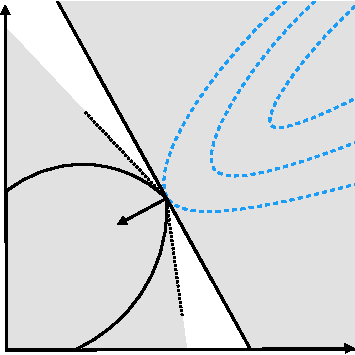
\includegraphics{part_2/chapter_7/figures/cones_F0_D.pdf}};	
		\node (S) at (-2, -1.5) {$S$};
		\node (D) at (-2.25, 1) {$D$};
		\node (F0) at (-1, 2.5) {$F_0$};
		\node (x0) at (0, -0.15) {$\overline{x}$};
			\node (gradfx0) at (-1.2, -0.4) {$\nabla f(\overline{x})$};					
	%					\draw[help lines] (-2,-2) grid (2,2);
	\end{tikzpicture}
	\caption{Illustration of the cones $F_0$ and $D$ for the optimal point $\overline{x}$. Notice that $D$ is an open set.} \label{cones_F0_D}
\end{figure}

As discussed earlier (in Lecture 4), in the presence of convex, this conditions becomes sufficient for optimality. Moreover, if $f$ is strictly convex, then $F = F_0$. If $f$ is linear, it might be worth considering $F_0' = \braces{d \neq 0 : \nabla f (\overline{x})^\top d \leq 0}$ to allow for considering orthogonal directions.

\subsection{Inequality constrained problems}

In mathematical programming applications, the feasibility set $S$ is typically expressed by a set of inequalities. Let us redefine $P$ as
%
\begin{align*}
	(P) :~ \mini \ & f(x)\\
	\st  &g_i(x) \leq 0, \ i=1,\dots,m\\
	&x \in X,
\end{align*}
%
where $g_i: \reals^n \mapsto \reals$, are differentiable functions for $i = 1, \dots, m$ and $X \subset \reals$ is an nonempty open set. The differentiability of $g_i$, $i=1, \dots, m$, allows for the definition of a proxy for $D$ using the gradients of the binding constraints $i \in I = \braces{i:g_i(\overline{x}) = 0}$ at $\overline{x}$. This set, denoted by $G_0$, is defined as
%
\begin{align*}
	G_0 = \braces{d : \nabla g_i(\overline{x})^\top d < 0, i \in I}.
\end{align*}
%
The use of $G_0$ is a convenient algebraic representation, since it can be shown that $G_0 \subseteq D$, which is stated in Lemma \ref{thm:G0_in_D}. As $F_0 \cap D = \emptyset$ must hold for a local optimal solution $\overline{x}\in S$, it follows that $F_0 \cap G_0 = \emptyset$ must also hold.
%
\begin{lemma}\label{thm:G0_in_D}
Let $S = \braces{ x \in X : g_i(x) \leq 0 \text{ for all } i=1,\dots,m}$, where $X \subset \reals^n$ is a nonempty open set and $g_i : \reals^n \rightarrow \reals$ a differentiable function for all $i = 1,\dots,m$. For a feasible point $\overline{x} \in S$, let $I = \braces{i:g_i(\overline{x}) = 0}$ be the index set of the binding (or active) constraints. Let
$$ G_0 = \braces{d : \nabla g_i(\overline{x})^\top d < 0, i \in I}$$
Then $G_0 \subseteq D$, where $D$ is the cone of feasible directions.
\end{lemma}
%
In settings in which $g_i$ is affine for some $i \in I$, it might be worth considering \lb $G_0' = \braces{d \neq 0: \nabla g_i (\overline{x})^\top d \leq 0, i \in I}$ so that orthogonal feasible directions can also be represented. Notice that in this case $D \subseteq G_0'$.


\section{Fritz-John conditions}

The Fritz-John conditions are the algebraic conditions that must be met for $F_0 \cap G_0 = \emptyset$ to hold. These algebraic conditions are convenient as they only involve the gradients of the binding constraints and they can be verified computationally.
%
\begin{theorem}[Fritz-John necessary conditions] \label{thm:FJ_conditions}
Let $X \subseteq \reals^n$ be a nonempty open set, and let $f:\reals^n \rightarrow \reals$ and $g_i:\reals^n \rightarrow \reals$ be differentiable for all $i = 1, \dots,m$. Additionally, let $\overline{x}$ be feasible and $I = \braces{i : g_i(\overline{x}) = 0}$. If $\overline{x}$ solves $P$ locally, there exist scalars $u_i$, $i \in \braces{0} \cup I$, such that
\begin{align*}
& u_0 \nabla f(\overline{x}) + \sum_{i=1}^m u_i \nabla g_i(\overline{x}) = 0\\
& u_i g_i(\overline{x}) = 0, \ i = 1,\dots,m\\
&u_i \geq 0, \ i = 0, \dots, m\\
&u = (u_0,\dots, u_m) \neq 0
\end{align*}
\end{theorem}
%
\begin{proof}
Since $\overline{x}$ solves $P$ locally, Theorem \ref{thm:geo_nec_cond} guarantees that there is no $d$ such that $\nabla f(\overline{x})^\top d < 0$ and $\nabla g_i(x)^\top d < 0$ for each $i \in I$. Let $A$ be the matrix whose rows are $\nabla f(\overline{x})^\top$ and $\nabla g_i(\overline{x})^\top$ for $i \in I$. 

Using Farkas' theorem, we can show that if $Ad < 0$ is inconsistent, then there exists nonzero $p \geq 0$ such that $A^\top p = 0$. Letting $p =(u_0, u_{i_1}, \dots, u_{i_{|I|}})$ for $I = \braces{i_1, \dots, i_{|I|}}$ and making $u_i = 0$ for $i \neq I$, the result follows. 
\end{proof}

The proof considers that, if $\overline{x}$ is optimal, then $f(\overline{x})^\top d \geq 0$ holds and a matrix $A$ formed by 
\begin{align*}
	A = \begin{bmatrix}
		\nabla f(\overline{x}) \\
		\nabla g_{i_1}(\overline{x})\\
		\vdots \\
		\nabla g_{i_|I|}(\overline{x})
	\end{bmatrix}
\end{align*}
with $I = \braces{i_1, \dots, i_{|I|}}$, will violate $Ad<0$. This is used with a variant of Farkas' theorem (known as the Gordan's theorem) to show that the alternative system $A^\top p = 0$, with $p \geq 0$ holds, which, by setting $p = [u_0, u_{i_1}, \dots, u_{i_|I|}]$ and enforcing that the remainder of the gradients $\nabla g_i(\overline{x})$, for $i \notin I$, are removed by setting $u_i = 0$, which leads precisely to the Fritz-John conditions.

The multipliers $u_i$, for $i=0,\dots,m$, are named Lagrangian multipliers due to the connection with Lagrangian duality, as we will see later. Also, notice that for nonbinding constraints ($g_i(\overline{x})<0$ for $i \notin I$), $u_i$ must be zero to form the Fritz-John conditions. This condition is named complementary slackness. 

% Include example from slides (ex_1) 

The Fritz-John conditions are unfortunately too weak, which is a problematic issue in some rather common settings. A point $\overline{x}$ satisfies the Fritz-John conditions if and only if $F_0 \cap G_0 = \emptyset$, which is trivially satisfied when $G_0 = \emptyset$.

For example, the Fritz-John conditions are trivially satisfied for points where some of the gradient vanishes (i.e., $\nabla f (\overline{x})=0$ or $\nabla g_i(\overline{x})=0$ for some $i=1,\dots,m$). Sets with no relative interior in the immediate vicinity of $\overline{x}$ also satisfy Fritz-John conditions. 

An interesting case is for problems with equality constraints, as illustrated in Figure \ref{FJ-linear}. In general, if the additional regularity condition that the gradients $\nabla g_i(\overline{x})$ are linearly independent does not hold, $\overline{x}$ trivially satisfies the Fritz-John conditions.

\begin{figure}[h]
	\begin{tikzpicture}
		\node (pic) at (0,0) {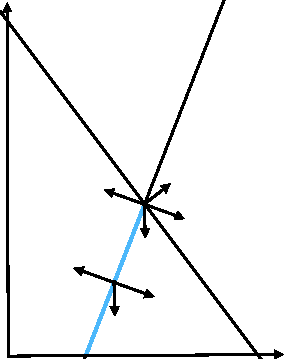
\includegraphics{part_2/chapter_7/figures/FJ_issue.pdf}};
		\node (x1)[above] at (2.4,-3) {\scriptsize$x_1$};
		\node (x2)[right] at (-2.3,2.95) {\scriptsize$x_2$};
		\node (nablaf1)[below] at (0.05,-0.9) {\scriptsize$\nabla f(\overline{x})$};
		\node (nablaf2)[below] at (-0.5,-2.2) {\scriptsize$\nabla f(x)$};
		\node (g1)[right] at (0.3,-0.1) {\scriptsize$\nabla g_1(\overline{x})$};
		\node (g21)[right] at (0.6,-0.7) {\scriptsize$\nabla g_2(\overline{x})$};
		\node (g22)[right] at (0.05,-2) {\scriptsize$\nabla g_2(x)$};
		\node (g31)[left] at (-0.6,-0.2) {\scriptsize$\nabla g_3(\overline{x})$};
		\node (g32)[left] at (-1.1,-1.5) {\scriptsize$\nabla g_3(x)$};
		\node (g1const)[right] at (0.2,-2.7) {\scriptsize$g_1(x) \le 0$};
		\node (g3const)[right] at (1,2) {\scriptsize$g_3(x) \le 0$};
		\node (g2const)[left] at (0.9,2) {\scriptsize$g_2(x) \le 0$};
	%			\draw[help lines] (-3,-3) grid (3,3);		
	\end{tikzpicture}
	\caption{All points in the blue segment satisfy FJ conditions, including the minimum $\overline{x}$.} \label{FJ-linear}
\end{figure}

 
\section{Karush-Kuhn-Tucker conditions}


The Karush-Kuhn-Tucker (KKT) conditions can be understood as the Frizt-John conditions with an extra requirement of regularity for $\overline{x} \in S$. This regularity requirement is called \emph{constraint qualification} and, in a general sense, are meant to prevent the trivial case $G_0 = \emptyset$, making thus the optimality conditions stronger (i.e., more stringent).

This is achieved by making $u_0 = 1$ in Theorem \ref{thm:FJ_conditions}, which ultimately implies that the gradients $\nabla g_i(\overline{x})$ for $i \in I$ must be linearly independent. This condition is called \emph{linearly independent constraint qualification} (LICQ) and is one of several known constraints qualifications that can be used to guarantee regularity of $\overline{x} \in S$. 

Theorem \ref{thm:KKT_conditions} establishes the KKT conditions as necessary for local optimality of $\overline{x}$ assuming that LICQ holds. For notational simplicity, let us assume for now that \begin{align*}
		(P) :~ \mini\braces{f(x) : g_i(x) \leq 0, i=1,\dots, m, x \in X}. 	
 	\end{align*}
%
\begin{theorem}[Karush-Kuhn-Tucker necessary conditions] \label{thm:KKT_conditions}
Let $X \subseteq \reals^n$ be a nonempty open set, and let \,$f:\reals^n \rightarrow \reals$ and $g_i:\reals^n \rightarrow \reals$ be differentiable for all $i = 1, \dots,m$. Additionally, for a feasible $\overline{x}$, let $I = \braces{i : g_i(\overline{x}) = 0}$ and suppose that $\nabla g_i(\overline{x})$ are linearly\hspace{-1pt} independent for all $i \in I$. If $\overline{x}$ solves $P$ locally, there exist scalars $u_i$ for $i \in I$ such that
\begin{align*}
& \nabla f(\overline{x}) + \sum_{i=1}^m u_i \nabla g_i(\overline{x}) = 0\\
& u_i g_i(\overline{x}) = 0, \ i = 1,\dots, m\\
& u_i \geq 0, \ i = 1, \dots, m 
\end{align*}
%
\end{theorem}
%
\begin{proof}
By Theorem \ref{thm:FJ_conditions}, there exists nonzero $(\hat{u}_i)$ for $i \in \braces{0} \cup I$ such that 
\begin{align*} 
& \hat{u}_0 \nabla f(\overline{x}) + \sum_{i=1}^m \hat{u}_i \nabla g_i(\overline{x}) = 0 \\ 
& \hat{u}_i \geq 0, \ i = 0, \dots, m
\end{align*}
Note that $\hat{u}_0 > 0$, as the linear independence of $\nabla g_i(\overline{x})$ for all $i \in I$ implies that $\sum_{i=1}^m \hat{u}_i \nabla g_i(\overline{x}) \neq 0$. Now, let $u_i = \hat{u_i}/u_0$ for each $i \in I$ and $u_i = 0$ for all $i \not\in I$. 
\end{proof} 
%
The proof builds upon the Fritz-John conditions, which under the assumption that the gradients of the active constraints $\nabla g_i (\overline{x})$ for $i \in I$ are independent, the multipliers $\hat{u}_i$ can be rescaled so that $u_0 = 1$.

The general conditions including both inequality and equality constraints are posed as follows. Notice that the Lagrange multipliers $v_i$ associated with the equality constraints $h(\overline{x}) = 0$ for $i=1, \dots,l$ are irrestricted in sign and the complementary slackness condition is not explicitly stated, since it holds redundantly. These can be obtained by replacing equality constraints $h(x) = 0$ with two equivalent inequalities $h_-(x) \leq 0$ and $-h_+(x) \leq 0$ and writing the conditions in Theorem \ref{thm:KKT_conditions}. Also, notice that, in the absence of constraints, the KKT conditions reduce to the unconstrained first-order condition $\nabla f(\overline{x}) = 0$. 
%
\begin{align*}
&\nabla f(\overline{x}) + \sum_{i=1}^m u_i \nabla g_i(\overline{x}) + \sum_{i=1}^{l} v_i \nabla h_i(\overline{x})= 0  &&\text{(dual feasibility 1)}\\ 
&u_i g_i(\overline{x}) = 0, \qquad~~\, i = 1,\dots,m &&\text{(complementary slackness)}\\
&\overline{x} \in X, \ g_i(\overline{x}) \leq 0, \ i = 1,\dots, m   &&\text{(primal feasibility)}\\
&h_i(x) = 0, \qquad\quad~~ i = 1,\dots, l\\
&u_i \geq 0, \qquad\qquad\quad i = 1, \dots, m &&\text{(dual feasibility 2)}
%$u \neq 0$ & (dual feasibility 3)
\end{align*}

The KKT conditions can be interpreted geometrically as follows. Consider the cone spanned by the active constraints at $\overline{x}$, defined as $N(\overline{x}) = \braces{\sum_{i \in I}u_i \nabla g_i(\overline{x}) : u_i \geq 0}$. A solution $\overline{x}$ will then satisfy the KKT conditions if $-\nabla f(\overline{x}) \in N(\overline{x})$, which is equivalent to $- \nabla f(\overline{x}) = \sum_{i=1}^m u_i \nabla g_i(\overline{x})$. Figure \ref{ex1_cone} illustrates this condition.

\begin{figure}
	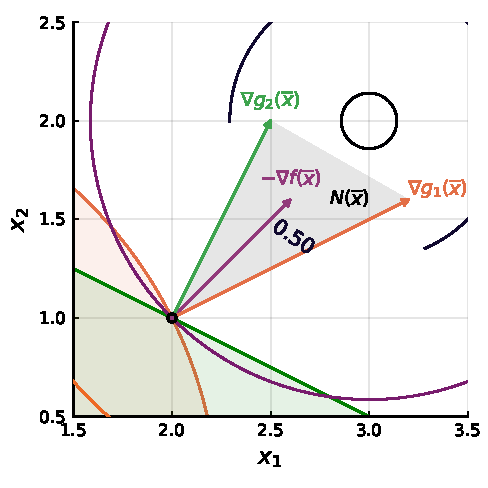
\includegraphics{part_2/chapter_7/figures/ex2_KKT.pdf}	
	\caption{Graphical illustration of the KKT conditions at the optimal point $\overline{x}$}\label{ex1_cone} 
\end{figure} 


\section{Constraint qualification}


Constraint qualification is a technical condition that needs to be assessed in the context of nonlinear optimisation problems. As we rely on an algebraic description of the set of directions $G_0$ that serves as proxy for $D$, it is important to be sure that the former is indeed a reliable description of the latter. 

In specific, constraint qualification can be seen as a certification that the geometry of the feasible region and gradient information obtained from the constraints that forms it are related at an optimal solution. Remind that gradients can only provide a \emph{first-order} approximation of the feasible region, which might lead to mismatches. This is typically the case when the feasible region has cusps, or a single feasible points. 

Constraint qualification can be seen as certificates for proper relationships between the set of feasible directions
\begin{align*}
G_0' = \braces{d \neq 0: \nabla g_i (\overline{x})^\top d \leq 0, i \in I}	
\end{align*}
%
and the cone of tangents (or tangent cone)
\begin{align}
	T = \braces{d : \ d = \lim_{k \rightarrow \infty}\lambda_k(x_k - \overline{x}), \lim_{k \rightarrow \infty}x_k = \overline{x}, 
            x_k \in S, \lambda_k > 0, \forall k} \label{eq:cone_tangents}
\end{align}
%
with $S = \braces{g_i(x) \leq 0, \ i = 1, \dots, m; h(x) = 0, \ i = 1, \dots, l; x \in X}$. 

The cone of tangents is a cone representing all directions in which the feasible region allow for an arbitrarily small movement from the point $\overline{x}$ while retaining feasibility. As the name suggests, it is normally formed by the lines that are tangent to $S$ at $\overline{x}$. Note that, however, if the point is in the interior of $S \subseteq \reals^n$, then $T = \reals^n$. 

One way of interpreting the cone of tangents as defined in  \eqref{eq:cone_tangents} is the following: consider a sequence of feasible points $x \in S$ in any trajectory you like, but in a way that the sequence converges to $\overline{x}$. Then, take the last (in a limit sense, since $k \rightarrow \infty$) $x_k$ and consider this direction from which $x_k$ came onto $\overline{x}$. The collection of all these directions from all possible trajectories is what forms the cone of tangents.  

Constraint qualification holds when $T = G_0'$ holds for $\overline{x}$, a condition named \emph{Abadie's constraint qualification}. In the presence of equality constraints, the condition becomes $T = G_0' \cap H_0$, with 
%
\begin{align*}
	H_0 = \braces{d: \nabla h_i(\overline{x})^\top d = 0, i =1, \dots, l}.
\end{align*} 
%
Figure \ref{fig:CQ-Tangent} illustrates the tangent cone $T$ and the cone of feasible directions ($G_0'$) for cases when constraint qualification holds (Figures \ref{fig:CG_ex1} and \ref{fig:CG_ex2}) for which case $T = G_0'$, and a case for when it does not (Figure \ref{fig:CG_ex3}, where $T = \emptyset$ and $G_0'$ is given by the dashed black line). 
%

\begin{figure}
		\begin{subfigure}{0.4\textwidth}
			\begin{tikzpicture}
				\node (pic) at (0,0) {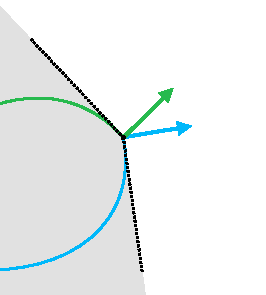
\includegraphics{part_2/chapter_7/figures/CG_ex1}};
				\node (T) at (-1.9,1.2) {\small $T = G_0'$};
				\node (S) at (-1.5,-0.5) {$S$};
				\node (x)[left] at (-0.1,0) {$\overline{x}$};
				\node (nablag1)[right] at (0.6,1) {$\nabla g_1(\overline{x})$};
				\node (nablag2)[right] at (0.9,0.3) {$\nabla g_2(\overline{x})$};
%				\draw[help lines] (-2,-2) grid (2,2);
			\end{tikzpicture}
			\caption{ }\label{fig:CG_ex1}
		\end{subfigure}
		\hspace{1cm}
		\begin{subfigure}{0.4\textwidth}
			\begin{tikzpicture}
				\node (pic) at (0,0) {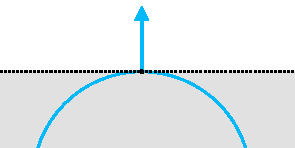
\includegraphics{part_2/chapter_7/figures/CG_ex2}};
				\node (T)[right] at (-2.2,-0.25) {\small $T = G_0'$};
				\node (S)[below] at (-0.1,-0.5) {$S$};
				\node (x)[below] at (-0.1,0.05) {$\overline{x}$};
				\node (nablag1)[right] at (-0.1,1) {$\nabla g_1(\overline{x})$};
%				\draw[help lines] (-2,-1) grid (2,1);
			\end{tikzpicture}
			\caption{ }\label{fig:CG_ex2}
				\begin{tikzpicture}
				\node (pic) at (0,0) {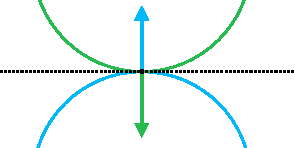
\includegraphics{part_2/chapter_7/figures/CG_ex3}};
				\node (T)[right] at (-2.5,-0.25) {\small $\emptyset = T \neq G_0'$};
%				\node (S)[below] at (-0.1,-0.5) {$S$};
				\node (x)[below] at (0.15,0.05) {$\overline{x}$};
				\node (nablag1)[right] at (-0.1,1) {$\nabla g_1(\overline{x})$};
				\node (nablag2)[right] at (-0.1,-1) {$\nabla g_2(\overline{x})$};
%				\draw[help lines] (-2,-1) grid (2,1);
			\end{tikzpicture}
			\caption{ }\label{fig:CG_ex3}
		\end{subfigure}
		\caption{CQ holds for \ref{fig:CG_ex1} and \ref{fig:CG_ex2}, since the tangent cone $T$ and the cone of feasible directions $G_0'$ (denoted by the dashed black lines and grey area) match; for \ref{fig:CG_ex3}, they do not match, as $T = \emptyset$}\label{fig:CQ-Tangent} \label{fig:CQ-Tangent}	
	\end{figure}


The importance of Abadie constraint qualification is that it allows for generalising the KKT conditions by replacing the condition the linear independence of the gradients $\nabla g_i(\overline{x})$ for $i \in I$. This allows us to state the KKT conditions as presented in Theorem \ref{thm:KKT_necII}.

\begin{theorem}[Karush-Kuhn-Tucker necessary conditions II] \label{thm:KKT_necII}
%
Consider the problem
$$(P) :~ \mini \braces{f(x) : g_i(x) \leq 0, i=1,\dots,m, x \in X}.$$
Let $X \subseteq \reals^n$ be a nonempty open set, and let $f:\reals^n \rightarrow \reals$ and $g_i:\reals^n \rightarrow \reals$ be differentiable for all $i = 1, \dots,m$. Additionally, for a feasible $\overline{x}$, let $I = \braces{i : g_i(\overline{x}) = 0}$ and \emph{suppose that Abadie CQ holds} at $\overline{x}$. If $\overline{x}$ solves $P$ locally, there exist scalars $u_i$ for $i \in I$ such that
\begin{align*}
& \nabla f(\overline{x}) + \sum_{i=1}^m u_i \nabla g_i(\overline{x}) = 0\\
& u_i g_i(\overline{x}) = 0, \ i = 1,\dots, m\\
&u_i \geq 0, \ i = 1, \dots, m. 
\end{align*}
%
\end{theorem}

Despite being a more general result, Theorem \ref{thm:KKT_necII} is of little use, as Abadie's  constraint qualification cannot be straightforwardly verified in practice. Alternatively, we can rely on verifiable constraint qualification conditions that imply Abadie's constraint qualification. Examples include 
%
\begin{enumerate}
\item {\bf Linear independence (LI)CQ:} holds at $\overline{x}$ if $\nabla g_i(\overline{x})$, for $i \in I$, as well as $\nabla h_i(\overline{x})$, $i = 1,\dots, l$ are \emph{linearly independent}.
\item {\bf Affine CQ:} holds for all $x \in S$ if $g_i$, for all $i=1,\dots,m$, and $h_i$, for all $i = 1,\dots, l$, are \emph{affine}.
\item {\bf Slater's CQ:} holds for all $x \in S$ if $g_i$ is a \emph{convex} function for all $i = 1,\dots,m$, $h_i$ is an \emph{affine} function for all $i = 1,\dots, l$, and there exists $x \in S$ such that $g_i(x) < 0$ for all $i = 1,\dots, m$.
\end{enumerate}
%
Slater's constraint qualification is the most frequently used, in particular in the context of convex optimisation problems. One important point to notice is the requirement of not having an empty relative interior, which can be a source of error. 

Consider, for example: $P = \braces{\mini x_1 : x_1^2 + x_2 \leq 0, x_2 \geq 0}$. Notice that $P$ is convex and therefore the KKT system for $P$ is 
$$ \binom{1}{0} + \begin{pmatrix} 0 & 0 \\ 1 & -1\end{pmatrix}\binom{u_1}{u_2} = 0; u_1,u_2 \geq 0,$$
which has no solution. Thus, the KKT conditions are not necessary for the global optimality of $(0,0)$. This is due to the lack of CQ, since the feasible region is the single point $(0,0)$ and the fact that KKT conditions are only sufficient (not necessary), in the presence of convexity.

Corollary \ref{thm:KKT_nec_suf} summarises the setting in which one should expect the KKT conditions to be necessary an sufficient conditions for global optimality, i.e., convex optimisation.

\begin{corollary}[Necessary and sufficient KKT conditions] \label{thm:KKT_nec_suf}
Suppose that Slater's CQ holds. Then, if $f$ is convex, the conditions of Theorem \ref{thm:KKT_necII} are \emph{necessary and sufficient} for $\overline{x}$ to be a global optimal solution. 
\end{corollary}
